\chapter{绪论}
自从进入21世纪,互联网已经不仅成为人类不可分割的一部分,也成为越来越多设备不可缺少的功能。人类和设备对上网带宽的需求越来越大,这促进了信息技术领域的高速发展。为了满足人类和设备日益增长的需求,光通信已经从主干网逐渐渗入到了房内。而在不远的将未来,光通信将迈向最后一步进入到处理器内部。而这对光通信的器件设备提出了新的要求。


传统光器件,虽然性能满足要求,但是由于其价格高,尺寸大,功耗大将无法满足大规模的应用。因此,研究人员从各方面不断尝试新的材料,新的结构探索高速,小尺寸,小功耗,价格低廉的解决方案。目前这个研究领域依旧热火朝天的进行着。


本章首先将介绍最有希望帮助光通信迈向最后一步的硅基光电子集成技术,接着着重讨论硅基光电子器件中的硅基光调制器,介绍其目前国内外的发展现状,最后将介绍在光调制器领域内由本作者首次完成的工作。


\section{硅基光电子集成技术的发展与现状}
随着信息技术的发展,短距离通信的速率不断提高。当数据的通信速率达到10 Gbps时,利用金属的电互联技术将会遇到能耗,串扰,损耗和电磁干扰等问题。尤其,面对当前云计算服务器间和多核处理器内,数据的交互需要在有限的空间内同时满足大带宽、低能耗和低成本的困境时,电互联的瓶颈凸显出来。电互联的这些缺点,可以通过光通信技术来解决。然而传统光通信由于单个光器件的成本高,集成度低,阻碍了传统光通信技术在短距离通信中的应用。

\begin{figure}[htb]
	\centering
	%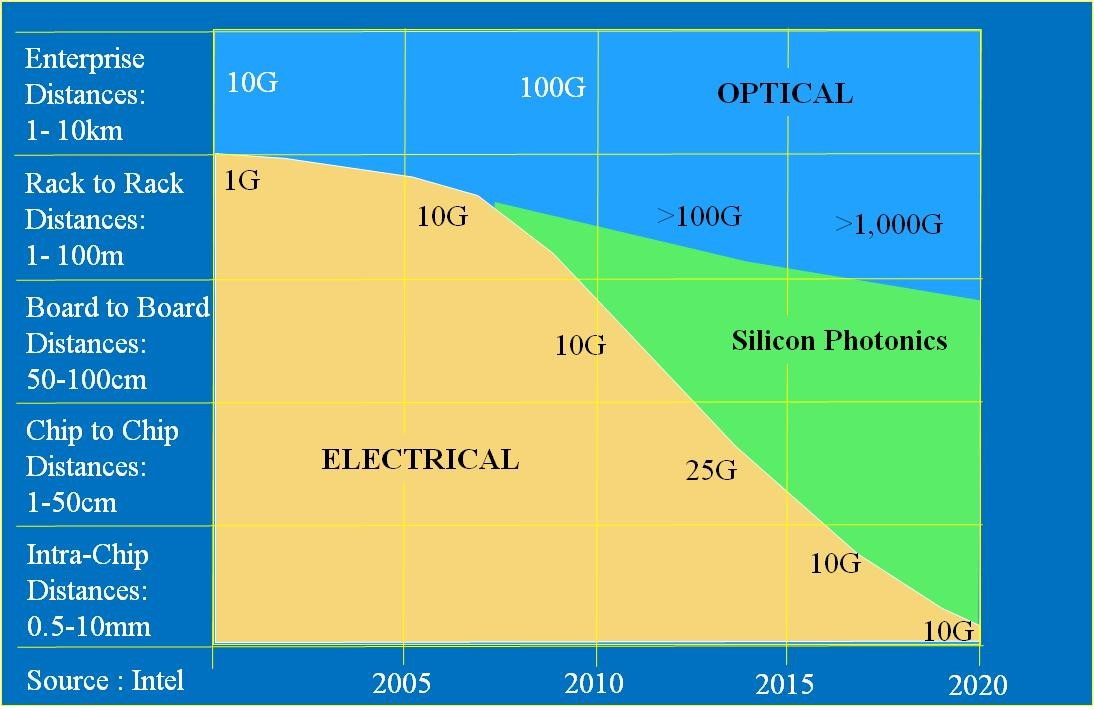
\includegraphics[width=\textwidth]{./Pictures/figure1.jpg}
	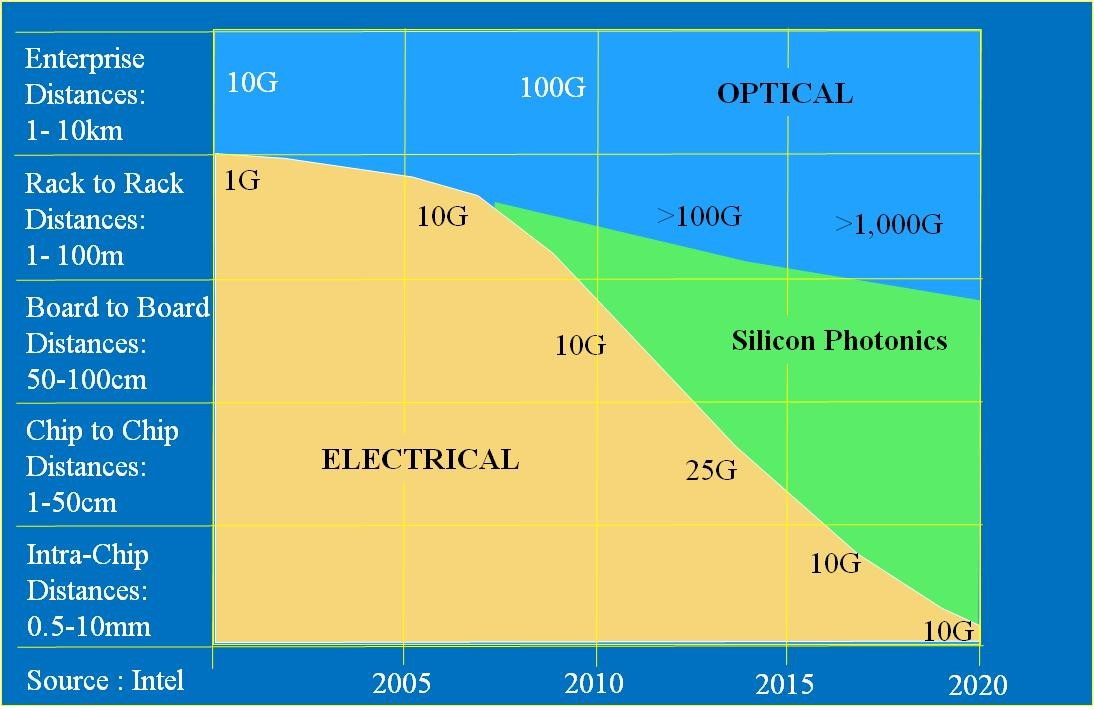
\includegraphics[width=12cm]{./Pictures/figure1.jpg}
	\caption{在不同通信距离下,电互联、硅基光通信和光纤通信的速率使用范围 \cite{Zuffada2012}}
	\label{figure1}
\end{figure}

(该段待续)硅基平台,即由硅衬底、二氧化硅绝缘层和硅薄膜构成的平台,不仅在传统半导体电子领域中有广泛运用,在微纳光子系统中也被广泛采用。硅基平台也成为了实现光电子集成芯片的理想平台。虽然,过去基于III-V材料的InP平台光电子平台已经实现了复杂的通信系统 ,但是大规模应用需要价格低廉,并且芯片间通信需要尺寸小,满足CMOS工艺。硅基光波导具有成本低,损耗低,折射率差大,结构小,的特别点。因此,硅基光电子平台越来在光通信领域受到人们的关注。

硅基光通信模块作为硅基光电子集成芯片的一个重要应用方向,其具有带宽大,功耗低,成本低的特点。图 \ref{figure1} 描述了电互联、硅基光通信和传统光纤通信和在不同距离下的适用速率范围 \cite{Zuffada2012}。图 \ref{figure1} 也预测了随着通信速率的逐年不断提高,硅基光通信在短距离将逐渐代替电互联。因此,硅基光集成芯片越来越收到各国的关注。美国在2004年率先提出了EPIC (Electronic and Photonic Integrated Circuits on Si)计划,研究硅基光电子集成平台,这将有助于通信,传感,微波光子学等研究方向的发展\cite{Shah2005}。欧洲在2008年提出了HELIOS (pHotonics ELectronics functional Integration on CMOS)计划,研究基于CMOS工艺的硅基光电子平台 \cite{HELIOS}。日本也紧跟而上,在2010年提出了PECST(Photonics and Electronics Convergence System Technology),推动硅基光电子平台的发展,实现芯片间的通信带宽密度达到10 Tb/s/cm\SP{2}\cite{Arakawa2013Silicon}。

光集成芯片的概念最早是由美国贝尔实验室的Miller在1969年提出来的\cite{miller1969}。随后1993, 美国空军科学研究实验室的Richard A. Soref提出了的硅基光电子集成芯片的概念\cite{Soref1993},见图 \ref{figure2} (a). 硅基光电子芯片是在同一片硅衬底上集成了负责逻辑和驱动的晶体管,负责光通信的激光器,调制器,光放大器,光探测器,光无源结构,光波导和光纤的耦合结构。在接下来的20多年内,全世界的知名高校和半导体公司都投入大量资金到这个领域中。在2011年,见图 \ref{figure2} (b), Intel厚积薄发推出了世界上第一个硅基光通信芯片包含了片上的激光器,纯硅调制器和硅锗探测器的光通信模块,实现了单通道12.5 Gbps的传输速率 \cite{Paniccia2011}。在2012年,见图 \ref{figure2} (c, d), IBM紧接发布了利用改进的90 nm CMOS工艺线,实现了在单个硅片上同时集成晶体管和的25 Gbps的光调制器和探测器 \cite{Assefa2012}。Intel虽然集成了激光器但是没能在单片上同时集成晶体管,而IBM虽然集成了晶体管,却没能集成激光器并且缺少完整光收发链路的展示。在2015年,美国伯克利大学和麻省理工大学的Chen Sun等首次展示了直接在商业化的45 nm CMOS流水线上,制作硅基光电子集成芯片 \cite{sun2015single}。该单块芯片,见图\ref{figure3} (a), 上不仅包含处理器,内存,还包含光收发模块。并且他们还展示了如图 \ref{figure3} (b) 所示的处理器的芯片和内存的芯片直接用光互联技术进行时时数据的运算和处理。虽然该硅基光电子芯片依旧缺少片上的激光器和放大器,但是该芯片是目前最复杂的单片硅基光电子芯片,包含了700万个晶体管和850个光模块。

\begin{figure}[htb]
	\centering
	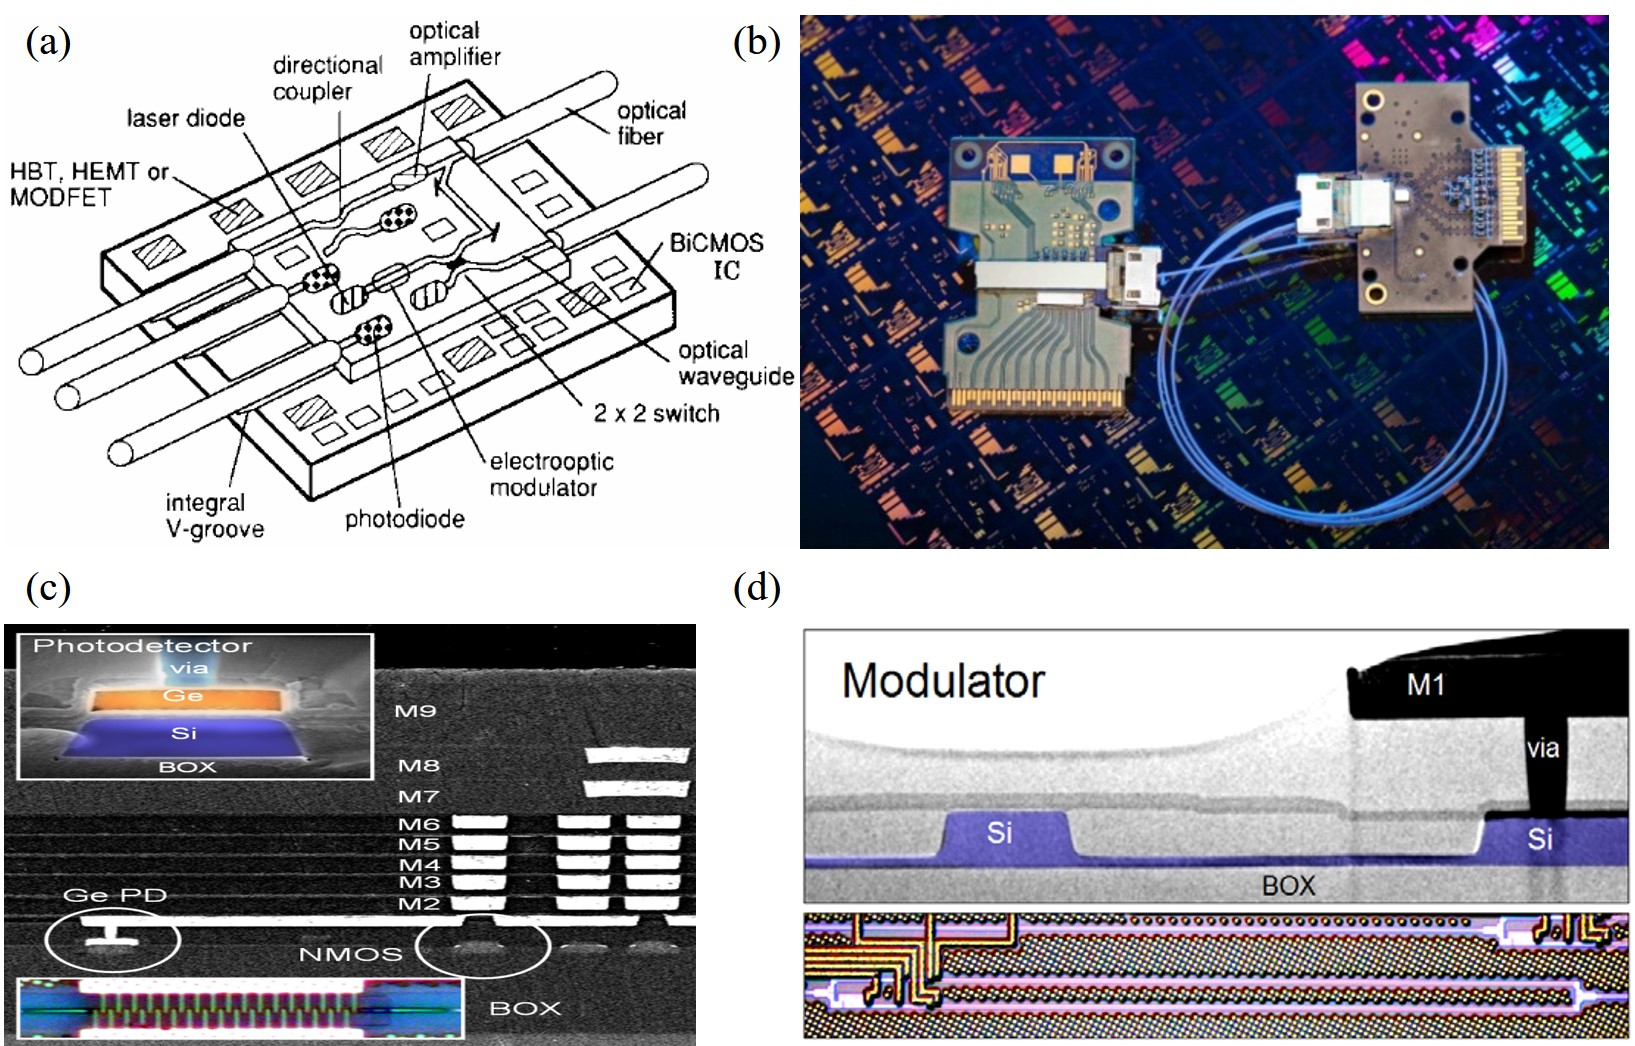
\includegraphics[width=12cm]{./Pictures/figure2.jpg}
	\caption{ (a) 最早的硅基光电子芯片概念图 \cite{Soref1993};(b)Intel的硅基光收发模块\cite{Paniccia2011};(c,d) IBM的硅基探测器和调制器\cite{Assefa2012}}
	\label{figure2}
\end{figure}

\begin{figure}[htb]
	\centering
	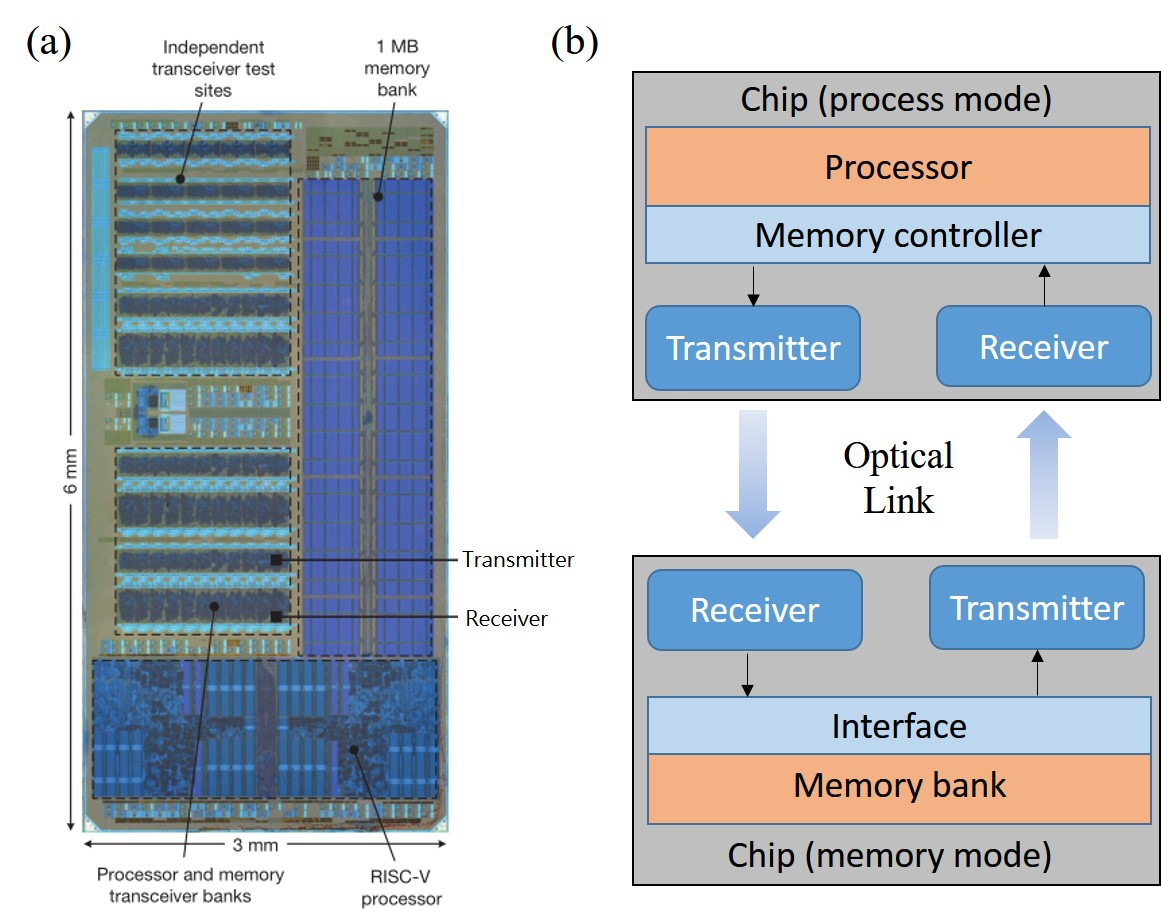
\includegraphics[width=10cm]{./Pictures/figure3.jpg}
	\caption{ (a) 单片硅基光电子芯片,包含处理器,内存,光收发模块\cite{sun2015single};(b) 处理器芯片和内存芯片间光互联示意图\cite{sun2015single}}
	\label{figure3}
\end{figure}

\section{硅基光调制器}
\subsection{硅基光调制器的指标}
\subsection{硅基光调制器的种类}

\section{论文的内容和创新点}

\subsection{论文内容}
\subsection{论文创新点}


